\Section{Background}

Summaries of everything required to understand the problem and its solution.

\begin{figure}[t]
    \centering
        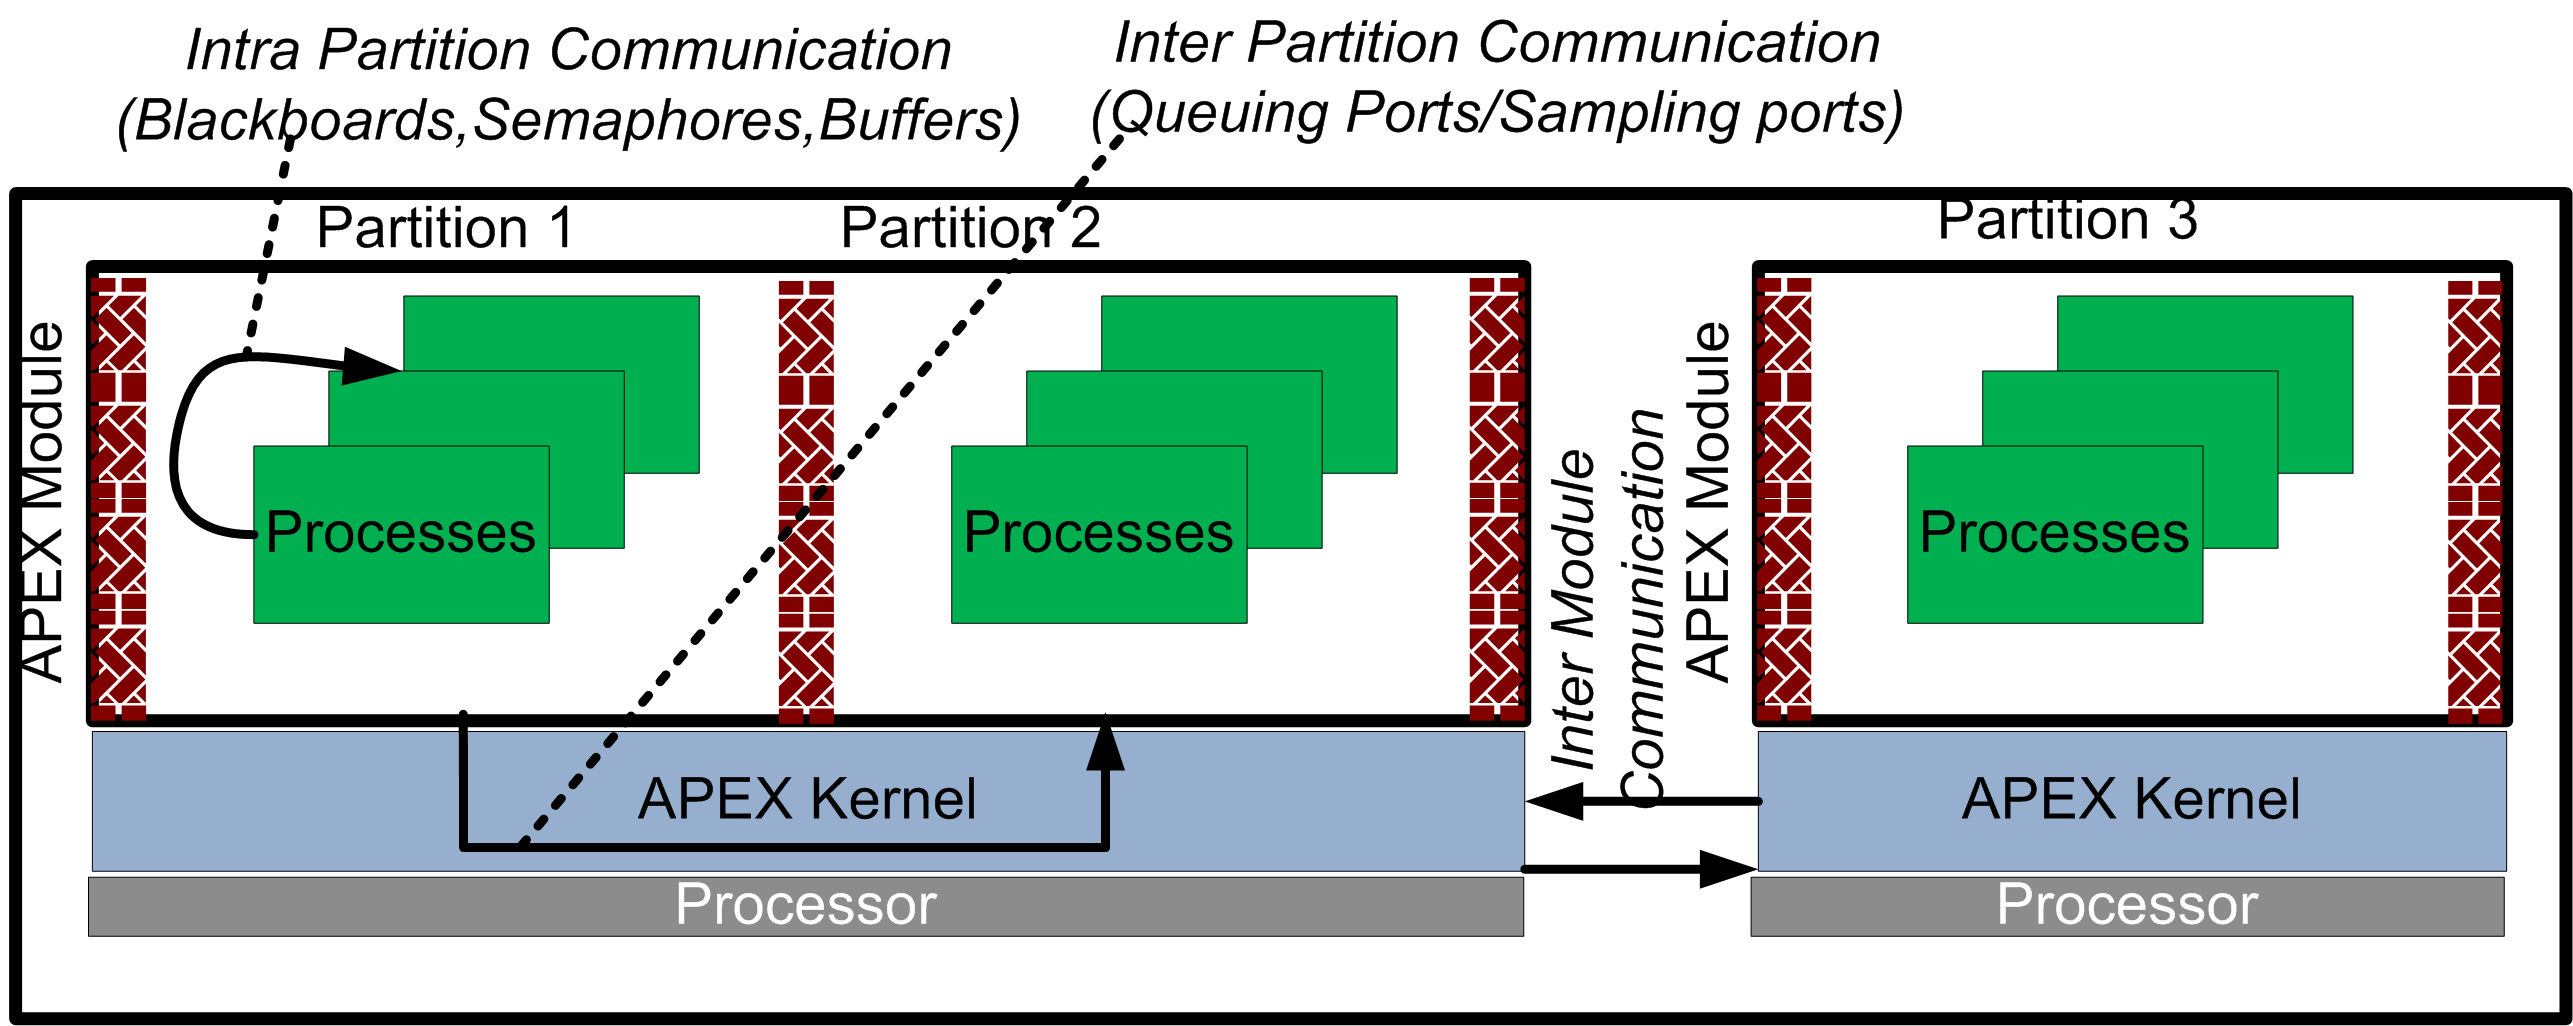
\includegraphics[width=\columnwidth]{figures/ARINC653.png}
    \caption{ ARINC 653 architecture.}
    \label{fig:653}
\end{figure} 

ARINC-653 software specification describes the standard Application Executive (APEX) kernel and associated services that are supported by safety-critical real-time operating systems (RTOS) used in avionics. ARINC-653 systems (see figure \ref{fig:653}) group {\it processes} into spatially and temporally separated \textit{partitions}, with one or more partitions assigned to each \textit{module}, and one or more modules (processor hosts) form a system.  While spatial partition guarantees total memory isolation between processes in two different partitions, temporal isolation ensures exclusive use of the processing resources by a partition. A fixed priority cyclic schedule is used by the RTOS to share the CPU between partitions. Within each partition, processes are scheduled in a priority preemptive manner. 

Processes within a partition share data only via the intra-partition services, and are responsible for their individual state. Intra-partition communication is supported using \textit{buffers} that provide a queue for passing data messages and \textit{blackboards} that allow processes to read, write and clear a single-item data message.    Inter-partition communication is asynchronous and is provided using ports and channels that can be used for \textit{sampling} or \text{queuing} of messages. 

Even though ARINC-653 specification provides a well-defined task execution model, it does not provide enough details about communication schedule. For example, there is no information and support for how a task execution model affects or is dependent upon the order in which the messages are sent over the shared bus. 


